\documentclass{article}
\usepackage[utf8]{inputenc}
\usepackage{graphicx}
\usepackage{float}
\usepackage{url}
\usepackage{hyperref}
\usepackage[margin=0.75in]{geometry}
\graphicspath{{./assets/}}

\title{Criterion B}
\author{Word count: 466}
\date{}

\begin{document}

\maketitle
\tableofcontents

\section{Technologies}

    \begin{itemize}
        \item \textbf{C++14} (g++ compiler)
            \begin{itemize}
                \item implementation language
                \item provides abstraction mechanisms without performance loss
            \end{itemize}
        \item \textbf{ASAN (ASan)} 
            \begin{itemize}
                \item debugging tool
                \item detects memory corruption (leaks, buffer and stack overflows)
            \end{itemize}
        \item \textbf{CMake}
            \begin{itemize}
                \item tool for generating makefiles 
                \item makes building larger C/C++ projects more efficient
            \end{itemize}
    \end{itemize}

\section{Test Plan}

    In order to test the interpreter, a series of programs testing features 
    described in success criteria have been written and will fed to the interpreter.
    [See Appendix B for source code of all tests] If the interpreter responses 
    as expected, test is passed. Additionally throughout the development address
    sanitizer is used to detect and mitigate memory leaks.


\section{General flowcharts}

    Flowcharts in case of an interpreter do not serve very important role in
    designing an tree-walk interpreter, as the main focus is on grammar, which 
    represented in flowcharts would grow to impractical sizes, similarly with
    the run-time logic of interpreter. This is why the flowcharts in this section
    represent general concepts.
    The program consists of three main stages: lexical analysis, parsing and 
    run-time. In Figure~\ref{fig:general_flow} there is a very general flowchart
    of the program. Green outlines point out that the process is more complex.
    \begin{figure}[H]
        \centering
        \caption{General flowchart of the program}
        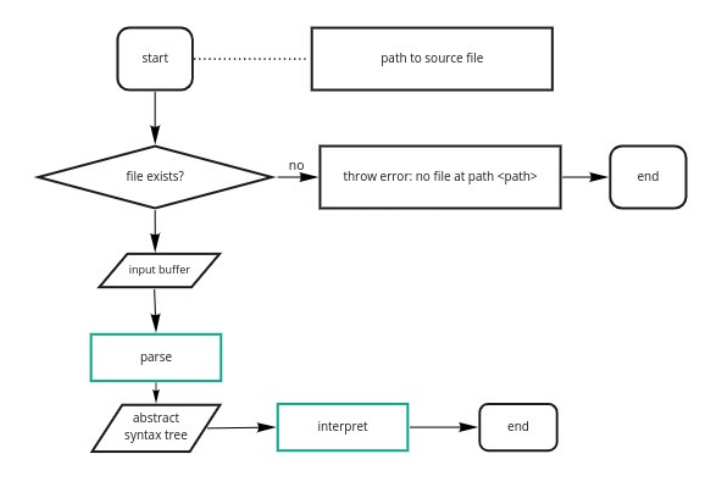
\includegraphics[width=\linewidth]{general_flowchart}
        \label{fig:general_flow}
    \end{figure}
    In Figure~\ref{fig:parser_flow} there is flowchart representing general
    idea behind recursive-descend parser. Parser uses lexer whose flowchart
    is in Figure~\ref{fig:lexer_flow}.
    \begin{figure}[H]
        \centering
        \caption{Flowchart of recursive-descend parser}
        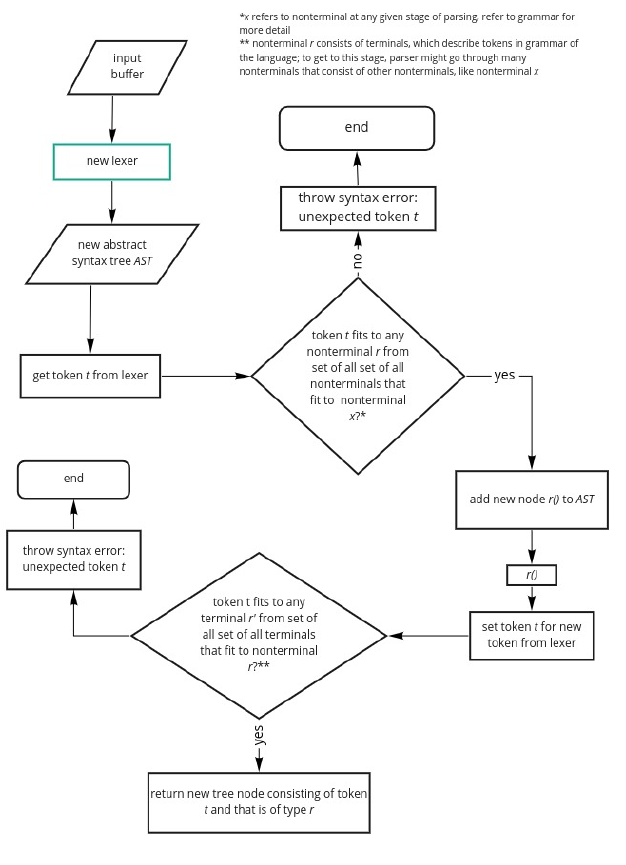
\includegraphics[width=\linewidth]{parser_flowchart}
        \label{fig:parser_flow}
    \end{figure}
    \begin{figure}[H]
        \centering
        \caption{Flowchart of lexer}
        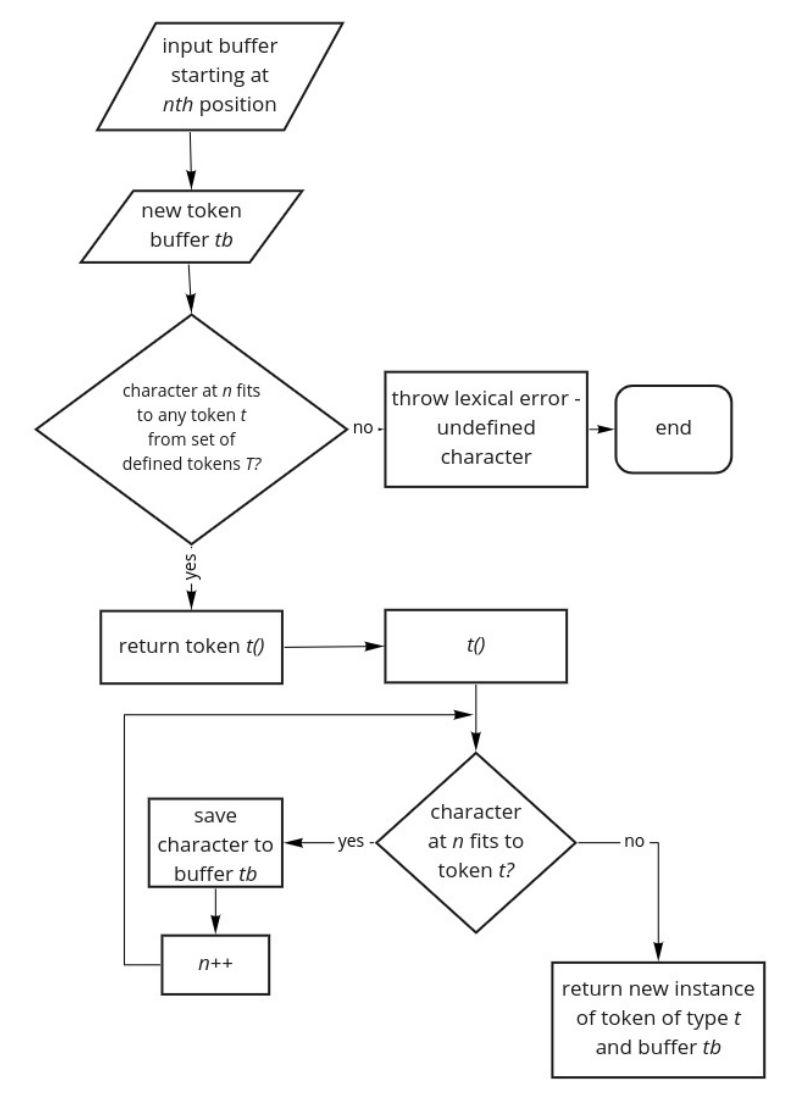
\includegraphics[width=\linewidth]{lexer_flowchart}
        \label{fig:lexer_flow}
    \end{figure}


\section{Language design}

\subsection{Tokens}

    Tokens represented in regular expressions, which also doubles as a blueprint 
    for lexer.

\begin{verbatim}
ID : [A-Z]([A-Z] | [0-9] | _)*
METHOD_ID : ([A-Z] | [a-z])[a-z]+ ([A-Z] | [a-z] | _)*
NUMBER : [0-9]+\.?[0-9]*
STRING : "."

RESERVED KEYWORDS / SYMBOLS:

method
if else then loop
while from to end
AND OR
+ - * / div %
< > >= <= == !=
( ) [ ]
\end{verbatim}


\subsection{Grammar}

    Backaus-Naur form (BNF) of IB pseudocode developed with reference to 
    pseudocode agenda made by IB\footnote{Link to source: %
    \url{https://ib.compscihub.net/wp-content/uploads/2015/04/IB-Pseudocode-rules.pdf}}
        . Since the parser is of recursive-descent type,
    each terminal reflects how the parser builds abtract syntax tree.

\begin{verbatim}
program :: block
         | block method
         | empty

method_decl :: METHOD METHOD_ID (param_decl) block END METHOD

param_decl  :: ID
             | ID, param_decl
             | empty

block   :: stmt block 
         | stmt
         | empty

stmt    :: assignment
         | if
         | for loop
         | while loop
         | method_call
         | expr
         | return
         | std_method
         | BREAK

assignment  :: ID = expr
             | ID = condition
             | ID = arr_decl
             | ID = arr_empty
             | ID = std_method
             | ID = STACK
             | ID = QUEUE

if  :: IF condition THEN block END IF
     | IF condition THEN block ELSE if END IF
     | IF condition THEN block ELSE if ELSE block END IF
     | IF condition THEN block ELSE block

for_loop    :: LOOP id FROM expr TO expr block END LOOP

while_loop  :: LOOP WHILE condition block END LOOP

method_call :: method_id(params) 

return  :: RETURN expr
         | RETURN condition
         | RETURN

params  :: list_of_elements

condition   :: cmp AND cmp
             | cmp OR cmp
             | cmp

cmp :: expr > expr
     | expr < expr
     | expr >= expr
     | expr <= expr
     | expr == expr
     | expr != expr

expr    :: term + term
         | term - term
         | term

term    :: factor * factor
         | factor / factor
         | factor DIV factor
         | factor MOD factor
         | factor

factor  :: NUM
         | STRING
         | ID
         | method_call
         | std_method
         | arr_acc
         | (expr)

arr_decl    :: [list_of_elements]
             | [arr_decl, arr_decl]

list_of_elements    :: expr
                     | expr, list_of_elements
                     | empty

arr_empty   :: ARRAY(list_of_elements)

arr_acc :: ID accessor

accessor    :: [NUM]
             | [NUM] accessor
             | empty

std_method  :: OUTPUT(params)
             | INPUT(STRING)
             | container_method

container_method    :: ID.length()
                     | ID.push()
                     | ID.pop(params)
                     | ID.enqueue(params)
                     | ID.dequeue()
                     | ID.getNext()

\end{verbatim}

\section{Inductive example of interpreter working with Abstract Syntax Tree (AST)}

    Suppose we have a very simple program:
    \begin{verbatim}
        A = 5
        if A == 5 then
            output("Hello, world!")
        end if
    \end{verbatim}
    After parsing, we would get the following AST - Figure~\ref{fig:AST}. The 
    red numbers beside nodes signify which node is being processed. 
    \begin{figure}[H]
        \centering
        \caption{Abstract Syntax Tree of the program}
        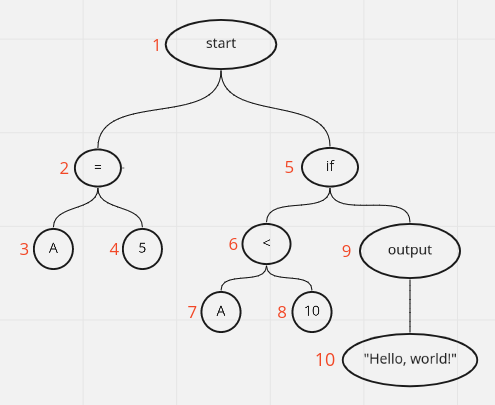
\includegraphics[width=0.5\linewidth]{AST}
        \label{fig:AST}
    \end{figure}
    Below is a ''transcript`` of what the interpreter does with the number referring
    to the number in the Figure~\ref{fig:AST}
    \begin{enumerate}
        \item start
        \item assign variable from right node to value from right node
        \item check if variable $A$ exists in activation record, if it does not,
            create a new field; return reference to the field
        \item return value reference to numerical value $5$
        \item check condition from right-most node, if it is true, then execute 
            other nodes
        \item if value from right node is lower than the one from left node, return
            true
        \item 
            \begin{itemize}
                \item check the type of node (here: variable)
                \item check activation record for variable $A$ - if it exists 
                    and is numerical
                \item return reference to numerical value of $A$
            \end{itemize}
        \item 
            \begin{itemize}
                \item check the type of node (numerical)
                \item return reference to numerical value $10$
            \end{itemize}
        \item print contents of the child node to the console
        \item return reference to a string \textit{``Hello, world!''}
    \end{enumerate}

    From this short example, it is apparent why flowcharts are not very applicable
    in design of the program, as each type of node holds a bit of different logic
    behind it.

\end{document}
